\documentclass[../notes.tex]{subfiles}
\begin{document}
\section{Day 3}
    \subsection{Products of Paths}
    \begin{itemize}
        \item \underline{Last time:} If $f$ and $g$ are any two paths in $\R^2$ from $p$ to $q$, then $f\cong_{p}q$.
        \item \underline{By contrast:} In, $S'=\{(x,y)\in \R^2| x^2+y^2=1\}$ if
            \begin{align*}
                f(s)&=(\cos(\pi s), \sin(\pi s))\\
                g(s)&=(\cos(\pi s), -\sin(\pi s))\\
            \end{align*}
            Then $f\ncong_{p}g$. (We'll prove this carefully later).
        \item \underline{Fact: (HW)} $\cong_{p}$ is an equivalence relation on the set $\{$paths in $X$ from $x$ to $y\}$
            Thus we can consider the set,
            \begin{align*}
                \faktor{\{ \text{paths in $X$ from $x$ to $y$}\}}{\cong_{p}}
                =\{\text{path-homotopy classes of paths in $X$ from $x$ to $y$}\}\ni [f]\\
            \end{align*}
            E.g. in the $S'$ example above, $[f]\neq[g]$
    \end{itemize}
        \begin{definition} Let the following be so,
            \begin{align*}
                X &=\ \text{topological space}\\
                f &=\ \text{path in $X$ from $x$ to $y$}\\
                g &=\ \text{path in $X$ from $y$ to $z$}\\
            \end{align*}\\
            Then the \underline{concatenation} of $f$ and $g$ is the path $f*g$ from $x$ to $z$ given by,
            \begin{align*}
                f*g:\ &I \rightarrow X\\
                (f*g)(s)&=\begin{cases}
                    f(2s) & \text{if}\ 0\leq s \leq \frac{1}{2}\\
                    g(2s) & \text{if}\ \frac{1}{2}\leq s \leq 1\\
                \end{cases}\\
            \end{align*}
        \end{definition}
        \begin{center}
        \begin{tikzpicture}
            \begin{axis}[ticks=none]
                \addplot[samples=200,domain=0:1,color=red,thick] {x^2}
                node [below right, pos=.5,color=red] {$f(s),\ s\in [0,1]$};
                \addplot[samples=200,domain=1:2,color=blue,thick] {2*x-1}
                node [above left,pos=.5,color=blue] {$g(s),s\in [0,1]$};
            \end{axis}
        \end{tikzpicture}
        \begin{tikzpicture}
            \begin{axis}[ticks=none]
                \addplot[samples=200,domain=0:1,color=magenta,thick] {x^2}
                node [above left, pos=1,color=magenta] {$(f*g)(s),\ s\in [0,1]$};
                \addplot[samples=200,domain=1:2,color=magenta,thick] {2*x-1};
                \draw [decorate, decoration={brace,
                                             amplitude=20pt,
                                             raise=2pt,
                                             mirror},color=cyan] (0,0) -- (100,100)
                     node [below right, pos=.4,yshift=-4.5mm, color=cyan] {{$0\leq s\leq \frac{1}{2}$}};
                \draw [decorate, decoration={brace,
                                             amplitude=20pt,
                                             raise=2pt,
                                             mirror},
                       color=orange] (102,102) -- (200,300)
                node [below right, pos=.4,yshift=-4.5mm, color=orange] {{$0\leq s\leq \frac{1}{2}$}};
            \end{axis}
        \end{tikzpicture}
        \end{center}
    \begin{itemize}
        \item Why is $f*g$ continuous?\\
        \begin{theorem}
            \underline{Gluing Lemma:} Let the following be so,
            \begin{align*}
                X &= \text{topological space}\\
                A,B \subseteq X,\ &\text{closed subsets such that } X=A\cup B\\
                Y &= \text{topological space}\\
            \end{align*}\\
            \begin{minipage}[c]{\linewidth}
                \begin{center}
                    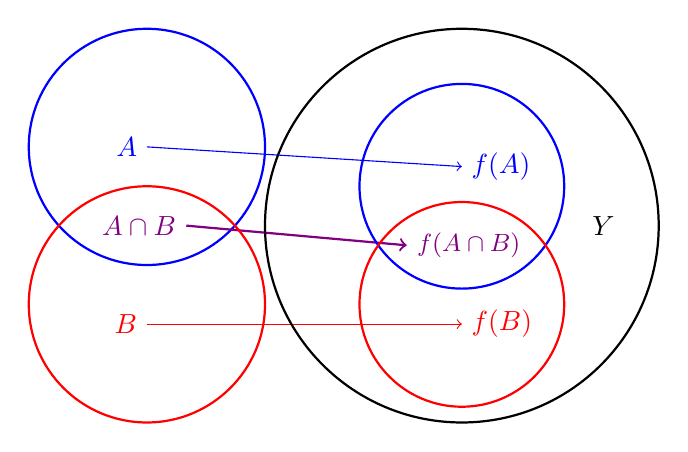
\begin{tikzpicture}
                        \draw [color=blue,thick] (2,3) circle(1.5cm);
                        \draw[->] [color=blue](2,3) node [left] {$A$} -- (6,2.75)
                        node [right]{$f(A)$};
                        \draw[->] [color=red](2,.75) node [left] {$B$} -- (6,.75)
                        node [right]{$f(B)$};
                        \draw[->] [color=violet,thick](2.5,2) node [left] {$A\cap B$} --
                        (5.3,1.75) node [right] {\small{$f(A\cap B)$}};
                        \draw [color=red,thick] (2,1) circle(1.5cm);
                        \draw [color=black,thick] (6,2) circle(2.5cm);
                        \draw (7.8,2) node [color=black,thick] {$Y$};
                        \draw [color=blue,thick] (6,2.5) circle(1.3cm);
                        \draw [color=red,thick] (6,1) circle(1.3cm);
                    \end{tikzpicture}
                \end{center}\\
            \end{minipage}\\ 
            \vspace{.5cm}\\
            Let the following continuous functions be defined,
            \begin{align*}
                f&:\ A \rightarrow Y\\
                g&:\ B \rightarrow Y\\
            \end{align*}
            such that $f(x)=g(x)\ \forall x \in A\cap B$.\\
            \vspace{.5cm}\\
            \begin{minipage}[c]{\linewidth}
                \begin{center}
                    \begin{tikzpicture}
                        \begin{axis}
                            [width=\linewidth,
                            height=5cm,
                            ymin=-1,ymax=1,
                            ticks=none]
                            \addplot [samples=200,color=blue,domain=0:1.25] {
                                .2*sin(deg(6.28*x))
                            }node [pos=0,below left] {$x$}
                            node [pos=.25,below] {$f(x)$}
                            node [pos=1, below] {$y$};
                            \addplot [samples=200,color=red,domain=.75:2] {
                                .2*sin(deg(6.28*x))
                            }node [pos=0,below] {$w$}
                            node [pos=.75, above] {$g(x)$}
                            node [pos=1, right] {$z$};
                            \draw [color=violet,decorate,decoration={brace,amplitude=5pt}]
                            (75,85) -- (120,130) node [above,pos=.5,yshift=3mm]
                            {$f(x)=g(x)$};
                        \end{axis};
                    \end{tikzpicture}
                \end{center}
            \end{minipage}\\
            \vspace{.5cm}\\
            Then the function,\\
            \begin{align*}
                h&:\ X\rightarrow Y\\
                h(x)&=\begin{cases}
                    f(x) & \text{if } x\in A\\
                    g(x) & \text{if } x\in B\\
                \end{cases}\\
            \end{align*}
            is continuous. The proof is left as an exercise to the reader. Thanks. (Homework Problem 1)\\
        \end{theorem}
            \underline{Note:} Applying the gluing lemma to $I = [0,\frac{1}{2}]\cup [\frac{1}{2}, 1]$ shows
            that $f*g$ is continuous.
        \item \underline{Question:} Let the following be so,
            \begin{align*}
                X &= \R^2\\
                f(s)&=(s-1,s)\\
                g(s)&=(s,s+1)\\
            \end{align*}
            What is $f*g$? Draw a picture.
        \item \underline{Answer:} 
            \begin{align*}
                f*g &= \begin{cases}
                    f(2s) & \text{if }0\leq s \le \frac{1}{2}\\
                    g(2s-1) & \text{if }\frac{1}{2}\leq s \le 1\\
                \end{cases}\\
            \end{align*}
            Which is a straight line from $(-1,0)$ to $(1,2)$.
        \item \underline{Proposition:} $*$ is well defined on path-homotopy classes of paths\\
            I.e., if,
            \begin{align*}
                f_0&\cong_{p}f_1\\
                g_0&\cong_{p}g_1\\
            \end{align*}
            then,
            \begin{align*}
                f_0*g_0\cong_{p}f_1*g_1\\
            \end{align*}
            This means that if $[f]=\{$path-homotopy equivalence class of f$\}$ then we can define,
            \begin{align*}
                [f]*[g]:=[f*g]\\
            \end{align*}
            as long as the end point of $f$ is the starting point of $g$.\\
            So, now $*$ is an operation.
            \begin{align*}
                \faktor{\{\text{ paths from $x\rightarrow y$}\}}{\cong_{p}}*\faktor{\{\text{paths $y \rightarrow z$}\}}{\cong_p}\rightarrow
                \faktor{\{\text{paths $x \rightarrow z$}\}}{\cong_{p}}\\
            \end{align*}\\
            \begin{minipage}[c]{\linewidth}
                \begin{center}
                    \includegraphics[width=\linewidth]{images/homotopy_class_concat.png}
                \end{center}
            \end{minipage}\\
            \begin{minipage}[c]{\linewidth}
                \begin{center}
                    \includegraphics[width=\linewidth]{images/homotopy_class_concat_2.png}
                \end{center}
            \end{minipage}
        \item \underline{Idea of proof of proposition:}\\
            Let,
            \begin{align*}
                F&:\ I\times I\rightarrow X \text{ be a path homotopy from $f_0$ to $f_1$}\\
                G&:\ I\times I\rightarrow X \text{ be a path homotopy from $g_0$ to $g_1$}\\
            \end{align*}
            Then we can define,
            \begin{align*}
                H&:\ I\times I \rightarrow X\\
                H(s,y)&=\begin{cases}
                    F(2s,t) & \text{if } 0\leq s \leq \frac{1}{2}\\
                    G(2s-1,t) & \text{if } \frac{1}{2}\leq s \leq 1 \\
                \end{cases}\\
            \end{align*}
            Then,
            \begin{align*}
                h_0=H(s,0)&=(f_0*g_0)(s)\\
                h_1=H(s,1)&=(f_1*g_1)(s)\\
                h_t=H(s,t)&=(f_t*g_t)(s) \text{ (some path between $x$ and $z$ )}\\
            \end{align*}
            So, $H$ is a path homotopy from $(f_0*g_0)$ to $(f_1*g_1)$.
    \end{itemize}
\end{document}
